\documentclass{article}
\usepackage[utf8x]{inputenc}
\usepackage{amsmath}
\usepackage[switch]{lineno} 
\usepackage{graphicx}
\usepackage{color}
\usepackage{url}
\usepackage{subcaption}
\usepackage{tabularx}
\usepackage{booktabs}
\usepackage[margin=1in]{geometry}
\usepackage{lineno}
\linenumbers

\newcommand{\beginsupplement}{%
        \setcounter{table}{0}
        \renewcommand{\thetable}{S\arabic{table}}%
        \setcounter{figure}{0}
        \renewcommand{\thefigure}{S\arabic{figure}}%
     }

\title{Is there an optimal management strategy for Amazonian production forests?}
\author{Camille Piponiot, Ervan Rutishauser, Plinio Sist,\\ TmFO author list, Bruno Hérault}
\date{}

\begin{document}

\maketitle 

\section{Abstract}

Tropical forests harbour most terrestrial carbon and diversity on Earth. Despite increased attention in national and international policies, they are still being deforested or degraded at high rates. 
In Amazonia, the largest tropical forest on Earth, a sixth of the remaining natural forests is dedicated to timber production. Conciliating timber production with the provision of other ecosystem services (ESs) remains a major challenge for forest managers and policy-makers. This study applies a spatial optimisation of logging in Amazonian production forests to analyse potential trade-offs between three ecosystem services, namely timber production, carbon storage and biodiversity conservation.  
Logging regulations currently applied in the region result in sub-optimal ES-use efficiency. Long-term timber provision would require adoption of a land-sharing strategy at regional scale (i.e. extensive logging with low intensities), whereas retention of carbon and diversity would be favoured in opting for a land-sparing strategy (i.e. intensive logging concentrated in the outer fringes of the Amazon region). Depending on management goals and societal demands, either choices are likely to have deep implications for the future of Amazonian forests. Overall, our results highlight the need for a reevaluation of current logging regulations and for regional cooperation among Amazonian countries to enhance coherent and trans-boundary forest management.

\twocolumn

\section{Introduction}


Tropical forests are of inestimable value for humanity. In addition to mitigating climate change by storing about 30\% of the terrestrial carbon \cite{Pan2013}, tropical forests also harbour half of the world biodiversity \cite{Pimm2014}, play a crucial role in regulating hydrological cycles \cite{Fisher2009a}, and furnish a wide range of timber and non-timber goods. Tropical forests are also the first source of new agricultural land, being converted at a higher-than-ever speed (2101 km$^2$ per year between 2000-2012 \cite{Hansen2013}); and the remaining forests are being increasingly degraded by human activities \cite{Potapov2017}. 

To tackle tropical deforestation, governments have long focused on forests conservation, mostly by setting up protected areas with restricted access and usage for human populations. However, this simple dichotomy (protected or not) poorly reflects the wide gradient of forest uses and their effects on tropical forests \cite{Gibson2011,DeCastroSolar2015}. As it is impossible to protect all tropical forests and unethical to ban humans, sustainable management aims at reconciling the conservation of forest functioning and health with sustained production of goods and services. 

In the tropics, c. 40\% of sawn wood traded annually arises from natural forests \cite{Payn2015}. Brazil is among the largest producers of tropical round wood, with 24 million m$^3$ (48\% of its production) of logs harvested annually (2005-2008) in natural tropical forests \cite{Blaser2011}. Selective logging is the dominant harvesting system in use, consisting in felling a few commercial trees and leaving the rest of the forest to natural dynamics. 
To avoid predatory logging practices that have depleted Amazonian forests of their most valuable timbers \cite{Richardson2016}, governments have implemented a set of logging rules, including minimum cutting cycles, i.e. time periods between two logging events (e.g., 20 years in Bolivia and Peru, 35 years in Brazil, and 65 years in French Guiana \cite{Blaser2011}), and maximum logging intensities ranging 20-30 m$^3$ha$^{-1}$, with an estimated mean logging intensity around 20~m$^3$ha$^{-1}$ in the Brazilian Amazon \cite{Asner2005}.

Because most of the forest cover remains after logging operations, selectively logged forests still harbour most of their initial carbon stocks, biodiversity, and other environmental features \cite{Putz2012}. It has frequently been argued that integrating selectively logged forests into tropical forest conservation schemes is of primary importance \cite{Edwards2014a}. Even though the value of production forests in providing Ecosystem Services (ESs) is increasingly recognised, trade-offs between ESs have rarely been investigated at large scale. Most conservation programs and payments for ES indeed focus on one particular feature (e.g. carbon in REDD+ programs \cite{Laing2016}), failing to account for forests multi-functionality and complexity \cite{VanderPlas2017}. Few studies have addressed multi-criteria decision-making in the context of tropical forests. For instance, a study in a logging concession in Suriname found that trade-offs between carbon stock conservation and timber recovery are mediated by logging intensity \cite{Roopsind2018}. Even though such studies provide useful insight for forest managers, they remain limited in scale, while most conservation-related policies apply at regional to national levels \cite{Hein2006b}. 

At the regional scale, natural production forests are managed to meet demands for high quality timber, while maintaining high levels of ES. To achieve such objectives, forest managers can choose between a continuum of 2 land use strategies: land sharing, which implies the use of less-damaging low-intensity logging on a large share of the landscape, or land sparing, which combines high-intensity logging with the preservation of most of the landscape \cite{Green2005}. 

Here we aim at optimising ES provision in Amazonian production forests in a spatially-explicit framework. We analyse the effect of different logging intensities (no logging or 10-20-30 m$^3$ha$^{-1}$) and cutting cycle duration (15-30-65 years) on the provision of three ES: timber recovery, carbon storage, and biodiversity conservation. Our main research questions are: (i) what are the best management choices for future production forests, (ii) what are the consequences of these management choices on ES provision, and (iii) how does the projected demand for high-quality timber affects forest management and associated ES provision? 

To answer these questions, we explore 8 management strategies (described in Table~\ref{tab:strategies}) and optimise ES with a timber production target of 35~Mm$^3$yr$^{-1}$, equivalent to the current timber production in Amazonia \cite{Lentini2005}. Strategies differ in terms of (i) ES prioritisation, (ii) total forest area allocated to production, (iii) whether total timber stocks must be recovered (i.e. sustainable timber yields) or not, and (iv) the application of a unique cutting cycle length (30 years). We compare the optimal spatial configuration of logging and resulting ES provision associated to each strategy. 
Finally, we analyse the consequences of changing the total timber production target depending on the management strategy.

\section{Materials and methods}

\subsection{Study region}

The study region is the Amazon region, located in tropical South America, mostly (60\%) in Brazil. Amazonia is the most diverse and carbon-rich tropical biome on Earth \cite{Avitabile2016,Pimm2014}, covered by around 600~Mha of tropical rainforest, of which 400~Mha are intact forests without detectable human footprint \cite{Potapov2017}. To date, 47\% of Amazonian forests is under legal protection \cite{WDPA2016} (Figure~\ref{fig:pharv}). However since the 1970' and the opening of the Transamazonian - the first road built deep inside the forest - 13.3\% of the original forest extent has been clearcut, mainly for agricultural purposes: cattle ranching and, more recently, soybean production \cite{Fearnside2017}. 

Even though Amazonia has already been deeply impacted by human activities and road building has continued steadily since the 1970', a great part of the biome is at a great distance from any road and thus inaccessible to most commercial activities (Figure~\ref{fig:pharv}).

Timber production through selective logging is the dominant forest use in the region, in terms of extent and generated income \cite{Blaser2011}. About 15\% of Amazonian forests is designated for timber production \cite{FAO2011}. If selectively logged forests still retain most of their original levels of carbon and diversity \cite{Putz2012}, forest recovery and resilience post-logging largely depend on implementation of logging in the field, the logging intensity and the cutting cycle length, \textit{i.e.} the time left to the forest to recover \cite{Rutishauser2015,Piponiot2018}. In Amazonia, logging intensities vary between 5-30~m$^3$ of timber extracted per ha, with an estimated average around 20~m$^3$ha$^{-1}$ in the Brazilian Amazon \cite{Asner2005}. Official minimum cutting cycle length varies from one country to another, ranging from 20 years (e.g. Peru, Bolivia \cite{Fredericksen2003,Blaser2011}) up to 65 years (French Guiana). 

\begin{figure}
    \centering
    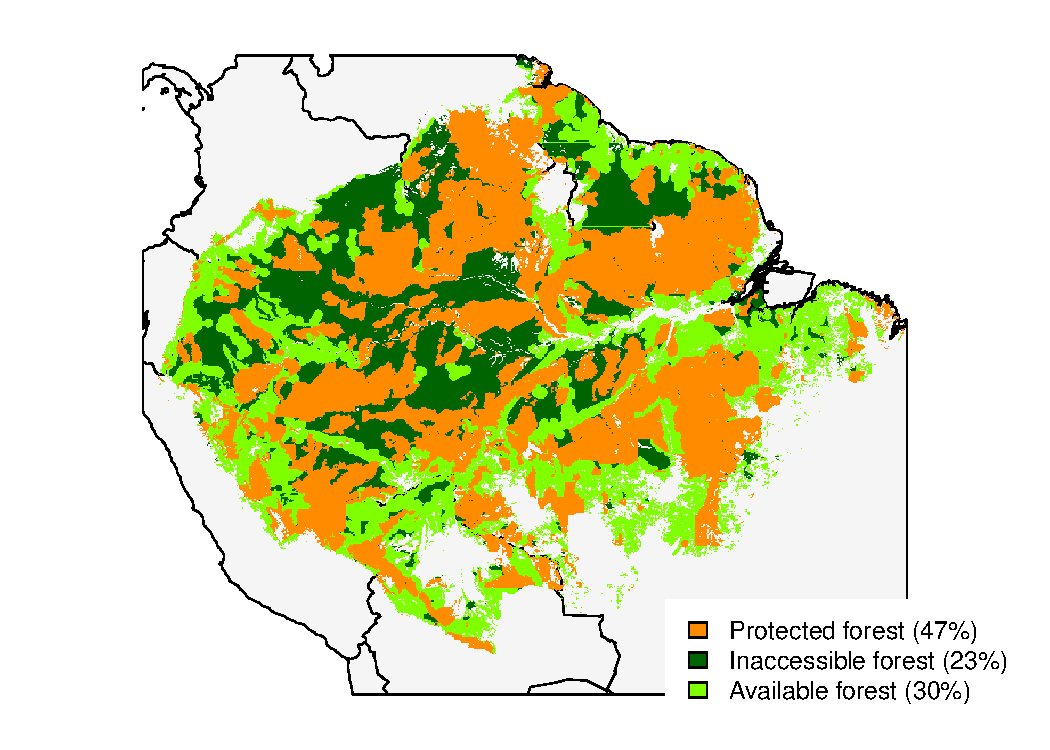
\includegraphics[width=\linewidth]{graphs/harv_areas.pdf}
    \caption{Availability of Amazonian forests for logging (forest cover $>$~90\%). Orange areas are protected areas (except category VI of the IUCN), and are not included in our analysis. Dark green areas are forests that are $>$ 25 km away from any road or track; light green areas are forests that are close ($\leq$ 25 km) to a road or track.}
    \label{fig:pharv}
\end{figure}


\subsection{Optimisation framework}

The goal of the optimisation is to find the best spatial configuration of different land uses in a landscape. In this study, Amazonia was divided into a systematic grid of 556 1$^{\circ}$ cells, which correspond to the coarsest resolution of input maps (see supplementary material~\ref{sec:defPPF}). 

The spatial optimisation seeks the most efficient spatial configuration of logging rules (cutting cycles and logging intensities) that minimises a cost function under pre-defined objectives. An annual timber production target is first set (Figure~\ref{fig:basicDiagram}): the optimal solution must include enough logged cells to produce the desired amount of timber. Then a management strategy is defined (see Table~\ref{tab:strategies} for a complete strategy description). The strategy includes (i) the weight of each ES (timber recovery, carbon storage and biodiversity conservation) in the cost function that will be minimised, (ii) the area of potential production forests (PPF) in each grid cell, and (iii) some additional constraints: sustainable timber yields (STY), unique cutting cycle length and intact forest landscape (IFL) conservation. 

The optimal spatial configuration for one given strategy is then found using a methodology adapted from the optimisation software \textit{Marxan with Zones} \cite{Watts2009}, using the package \textit{prioritzr} \cite{Hanson2018} developed in R programming language \cite{RCoreTeam2017}. Codes are available at [link XXX - \url{github.com/cpiponiot/ES_optimisation_Amazonia}]. 

\begin{figure}
    \centering
    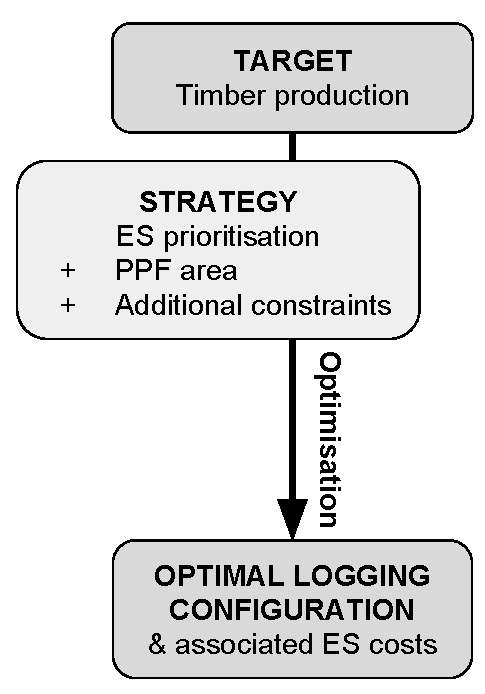
\includegraphics[width = 0.6\linewidth]{graphs/diagramSpatOptim}
    \caption{Diagram of spatial optimisation steps. PPF: Potential Production Forests, i.e. all forests that are accessible and where logging is allowed. The 8 strategies tested in this study are summarised in Table~\ref{tab:strategies}. The resulting logging configuration and associated changes in ES provision with a 35~Mm$^3$yr$^{-1}$ are presented in Figures~\ref{fig:mapsStrateg} and \ref{fig:scenESProv}, respectively. The effects of changing the timber production target are presented in Figure~\ref{fig:incDemand}.}
    \label{fig:basicDiagram}
\end{figure}

\subsection{Strategy description}

Different strategies to supply future timber demand in the region (Table~\ref{tab:strategies}) are tested: (i) \textit{Timber}: only timber recovery is optimised in order to ensure long-term timber production, (ii) \textit{Carbon}: only carbon is optimised as a climate change mitigation strategy, (iii) \textit{Biodiversity}: only biodiversity is optimised as a conservation strategy, (iv) \textit{Balanced}: long-term timber provision and conservation values (carbon and biodiversity) are balanced in the optimisation, as a multifunctionality strategy, (v) \textit{Current}: balanced ES prioritisation under medium (30-yr) cutting cycles, (vi) \textit{STY}: sustained timber yields (STY), i.e. the volume of timber extracted must be recovered at the end of the first cutting cycle, (vii) \textit{Road building}: all areas, except currently-protected areas, are made available for logging, and (viii) \textit{STY - Road building}: all areas, except currently-protected areas, are made available for STY logging. Both strategies involving the expansion of new roads mirror a land-sharing strategy. For the Timber strategy, total timber harvested can vary between 10-80~Mm$^3$yr$^{-1}$ (Figure~\ref{fig:incDemand}), but 80\% of IFL is maintained. Such an intensification of timber production in current production forests rather reflects a land-sparing approach.

In scenarios (i-v), the area suitable for logging is the same as defined previously (\textit{Currently accessible} in Table~\ref{tab:strategies}). In the \textit{Road building} scenarios (v-vi), we hypothesise that additional roads will be built: the new area suitable for logging (\textit{All unprotected} in Table~\ref{tab:strategies}) corresponds to the total area with forest cover $>$~90\% outside protected areas (independently of their current distance to a road), minus the 42\% corresponding to slopes and areas near rivers (see section~\ref{sec:ppf}). 

\begin{table*}
    \centering
    \begin{tabularx}{\textwidth}{p{2cm} p{4.5cm} p{2cm} p{3.5cm} p{0.8cm} p{1cm}}
    \toprule
         Acronym & Strategy & ES prioritisation & PPF area &  STY & 30-yr cycle \\
         \midrule
         Timber & Long-term timber production & Timber  & Currently accessible & No & No\\
         Carbon & Climate change mitigation &  Carbon & Currently accessible & No & No\\
         Biodiversity & Biodiversity conservation &  Biodiversity & Currently accessible & No & No \\
         Balanced & Multi-functionality & Balanced & Currently accessible & No & No \\
         Current & Only 30-yr cutting cycles & Balanced & Currently accessible & No & Yes \\
         STY & Sustained timber yields & Balanced & Currently accessible & Yes & No \\
         Road building & Building roads to previously inaccessible areas & Balanced & All unprotected & No & No \\
         STY + Road building & Sustained timber yields with road building & Balanced & All unprotected & Yes & No \\
         \bottomrule
    \end{tabularx}
    \caption{Strategies tested in this study. ES prioritisation refers to the weights given to ESs in the optimisation process: either only one ES (timber, carbon or biodiversity) is optimised, or weights are balanced between timber and conservation (carbon and biodiversity). PPF (potential production forests) are areas that can be logged in a given strategy: "Currently accessible" are areas that have $>$~90\% forest cover, are not protected and are within 25~km of an existing road or track (Figure~\ref{fig:pharv}); "All unprotected" are all areas with $>$~90\% forest cover outside protected areas (no road-distance restriction). Two optional constraints can be added: STY (Sustained Timber Yields) requires that the total timber stocks are recovered over all logged grid cells; the 30-yr cycle constraint allows only 30-yr cutting cycles.}
    \label{tab:strategies}
\end{table*}

\subsection{ES prioritisation}

Spatially-explicit logging costs are estimated as the loss of each ES (i.e. carbon emissions, biodiversity loss, and timber stocks decrease) caused by logging operations and are calculated in each grid cell.

To reflect the range of practices currently in use in the region, logging could take one of the following feature: a logging intensity of 10 (Low), 20 (Medium) or 30 (High) m$^3$ha$^{−1}$, and a cutting cycle length of 15 (Short), 30 (Medium) or 65 (Long) years, or no Logging. Medium intensity and cutting cycle length correspond to current median logging practices in Amazonia. 

The total cost of allocating logging type $z$ to grid cell $p$ is estimated as: 

\begin{equation}
\begin{split}
    Cost_{p,z} = \alpha _T \cdot \frac{Prod_{p,z} - Rec_{p,z} - K}{\overline{Prod - Rec - K}} \\+ \alpha _C \cdot \frac{Cemi_{p,z}}{\overline{Cemi} }  + \alpha _B \cdot \frac{Rloss_{p,z}}{\overline{Rloss}} 
\end{split}
\end{equation}

where $\alpha_T$, $\alpha_C$ and $\alpha_B$ are the relative weights of timber, carbon and biodiversity respectively. 
$Prod_{p,z}$ is the timber extracted in a grid cell $p$ when allocated to logging type $z$ and $Rec_{p,z}$ is the timber recovered at the end of the cutting cycle \cite{Piponiotc}: $Prod_{p,z} - Rec_{p,z}$ is thus the net timber loss. A constant $K$ was added to avoid negative costs (when timber recovery exceeds timber extraction). $K$ is set to the minimum cost value across all grid cells and all logging types. 
$Cemi_{p,z}$ are the total carbon emissions caused by logging operations (log extraction, road opening and incidental damage) minus the carbon recovered after logging \cite{Piponiot2016a}, integrated over the first cutting cycle period.
$Rloss_{p,z}$ are vertebrates species loss (mammals and amphibians \cite{Jenkins2013}) at the end of the first cutting cycle in a grid cell $p$ when allocated to logging type $z$. 
ES losses are standardised by their respective sample mean $\overline{Cemi}$, $\overline{Rloss}$, and $\overline{Prod-Rec-K}$. 

When a unique ES (timber, carbon or biodiversity) is prioritised in a given strategy, its weight is set to 1 and the other 2 are set to 0. When ES prioritisation is balanced between production and conservation, $\alpha_T = 0.5$ and $\alpha_C = \alpha_B = 0.25$.

To analyse the effect of ES prioritisation on final ES costs, we ran 66 simulations with all combinations of weights from 0 to 1, with 0.1 steps. Results are analysed in the Supplementary material (Section~\ref{supsec:changeCost}, Figure~\ref{fig:changeCosts}).  

\subsection{Potential Production Forest area}
\label{sec:ppf}

The total area of a grid cell ranged from 1.17 to 1.23 Mha. In each grid cell, we considered only areas suitable for logging, referred to as "potential production forests" (PPF). The area of all unprotected PPF was estimated as areas (i) having at least 90\% of forest cover \cite{Hansen2013}, and (ii) not being under a full protection status \cite{WDPA2016}. To estimate the currently accessible PPF area, the areas that are more than 25~km away from any road or motorable track were removed \cite{OSM2018}. Additional information is provided in the Supplementary material (Section~\ref{sec:defPPF}). 

The total areas of PPF ("all unprotected" and "currently available") are then calculated for each grid cell. Because part of a production forest area is considered as unsuitable for logging (slopes, areas around rivers and streams, etc) \cite{Verissimo2006}, the total area of PPF was multiplied by a coefficient $\pi = 58\%$, calibrated with data from French Guiana concessions \cite{Piponiotc}. 

\subsection{Additional constraints}

\subsubsection{Sustainable timber yields}

An optional sustainable timber yields (STY) constraint was added to the \textit{STY} and \textit{STY + Road building} strategies. In these strategies, timber recovery over all grid cells must be greater or equal to harvested timber volumes: 

\begin{equation}
    \sum_{p}\sum_{z} (Rec_{p,z} - Prod_{p,z}) \geq 0 
\end{equation}
where $Prod_{p,z}$ and $Rec_{p,z}$ area respectively the harvested and recovered timber in grid cell $p$ allocated to logging type $z$.

\subsubsection{Unique cutting cycle length}

In the "Current" strategy, grid cells can be allocated to only 4 logging types: 30-year cutting cycles (Medium) with 10-, 20- or 30-m$^3$ha$^{-1}$ logging intensities, or no logging. 

\subsubsection{IFL conservation}

Finally, an additional constraint  to conserve biodiversity is added to all strategies: it consists in conserving most intact forest landscapes (IFL). IFL are irreplaceable for biodiversity conservation \cite{Gibson2011}, especially for species that are highly sensitive to forest degradation. Because Amazonian forests have high levels of endemism and all regions are not equivalent in terms of species composition, we defined the biodiversity conservation objective as follow: in each of the 6 ecoregions (according to ter Steege et al. \cite{TerSteege2013}), namely the Guiana Shield, eastern Amazon, southeastern Amazon, central Amazon, southwestern Amazon, and northwestern Amazon, 80\% of IFLs (according to Potapov et al. \cite{Potapov2017}) shall remain unlogged. Those include forests in protected areas, inaccessible forests ($>$ 25 km from a road or track), or forests inside grid cells that have been allocated to the "No Logging" type. 

\section{Results}

\subsection{Optimal logging configuration under current timber production target}

Minimising timber loss (i.e. the \textit{Timber} strategy) results preserving only 10\% of the available area while logging 12\% under high-intensity short-cycle logging and 77\% under low-intensity (10~m$^3$ha$^{-1}$) long-cycle (65 yr) logging. Low-intensity logging is distributed in almost every region of Amazonia, except in the northeast where high-intensity logging prevails (Figure~\ref{fig:mapsStrateg}a). 
By contrast, maximising carbon and biodiversity retention results in preserving 82\% of available forests, and logging 18\% of available forests under the highest intensity (30~m$^3$ha$^{-1}$) and shortest cutting cycle (15 yr) allowed (Figure~\ref{fig:mapsStrateg}b-c). Logged areas are distributed in the most external areas of Amazonia: in southeastern Amazonia for both carbon and biodiversity, in northern Amazonia for carbon and in the southwestern border of Amazonia for biodiversity.  

Balancing timber, carbon and biodiversity optimisation results in preserving 48\% of available forests, logging 15\% of available forests under high-intensity (30~m$^3$ha$^{-1}$) short-cycle (15 yr) logging and 36\% under low-intensity (10~m$^3$ha$^{-1}$) long-cycle (65 yr) logging (Figure~\ref{fig:mapsStrateg}d). Similar to the \textit{Carbon} and \textit{Biodiversity} strategies, heavily logged areas are concentrated in most external areas, especially in the southeastern border; low-intensity logging is concentrated in the south and northwest; central, western and northeastern Amazonia are mostly not logged. 

Allowing only 30-yr cutting cycles results in preserving a smaller share of available forests (35\%) while 22\% are logged under high-intensity (30 m$^3$ha$^{-1}$) logging and 43\% under low-intensity (10 m$^3$ha$^{-1}$) logging (Figure~\ref{fig:mapsStrateg}e). 

Adding a STY constraint (Figure~\ref{fig:mapsStrateg}f) results in very little change compared to the \textit{Balanced} strategy. A slightly higher proportion (39\% instead of 36\%) of areas are logged under low-intensity (10~m$^3$ha$^{-1}$) long-cycle (65 yr) logging; this results in fewer preserved areas (45\% instead of 48\%). 

Increasing the total accessible forest area through road building (Figure~\ref{fig:mapsStrateg}g) also results in a spatial configuration similar to the \textit{Balanced} strategy. The total area under high-intensity (30~m$^3$ha$^{-1}$) short-cycle (15 yr) logging is slightly lower than in the \textit{Balanced} strategy (13~Mha instead of 15~Mha) and the total area under low-intensity (10~m$^3$ha$^{-1}$) long-cycle (65 yr) logging is higher (55~Mha instead of 35~Mha). Adding a STY constraint did not change the final results (Figure~\ref{fig:mapsStrateg}h). 

\begin{figure*}
    \centering
    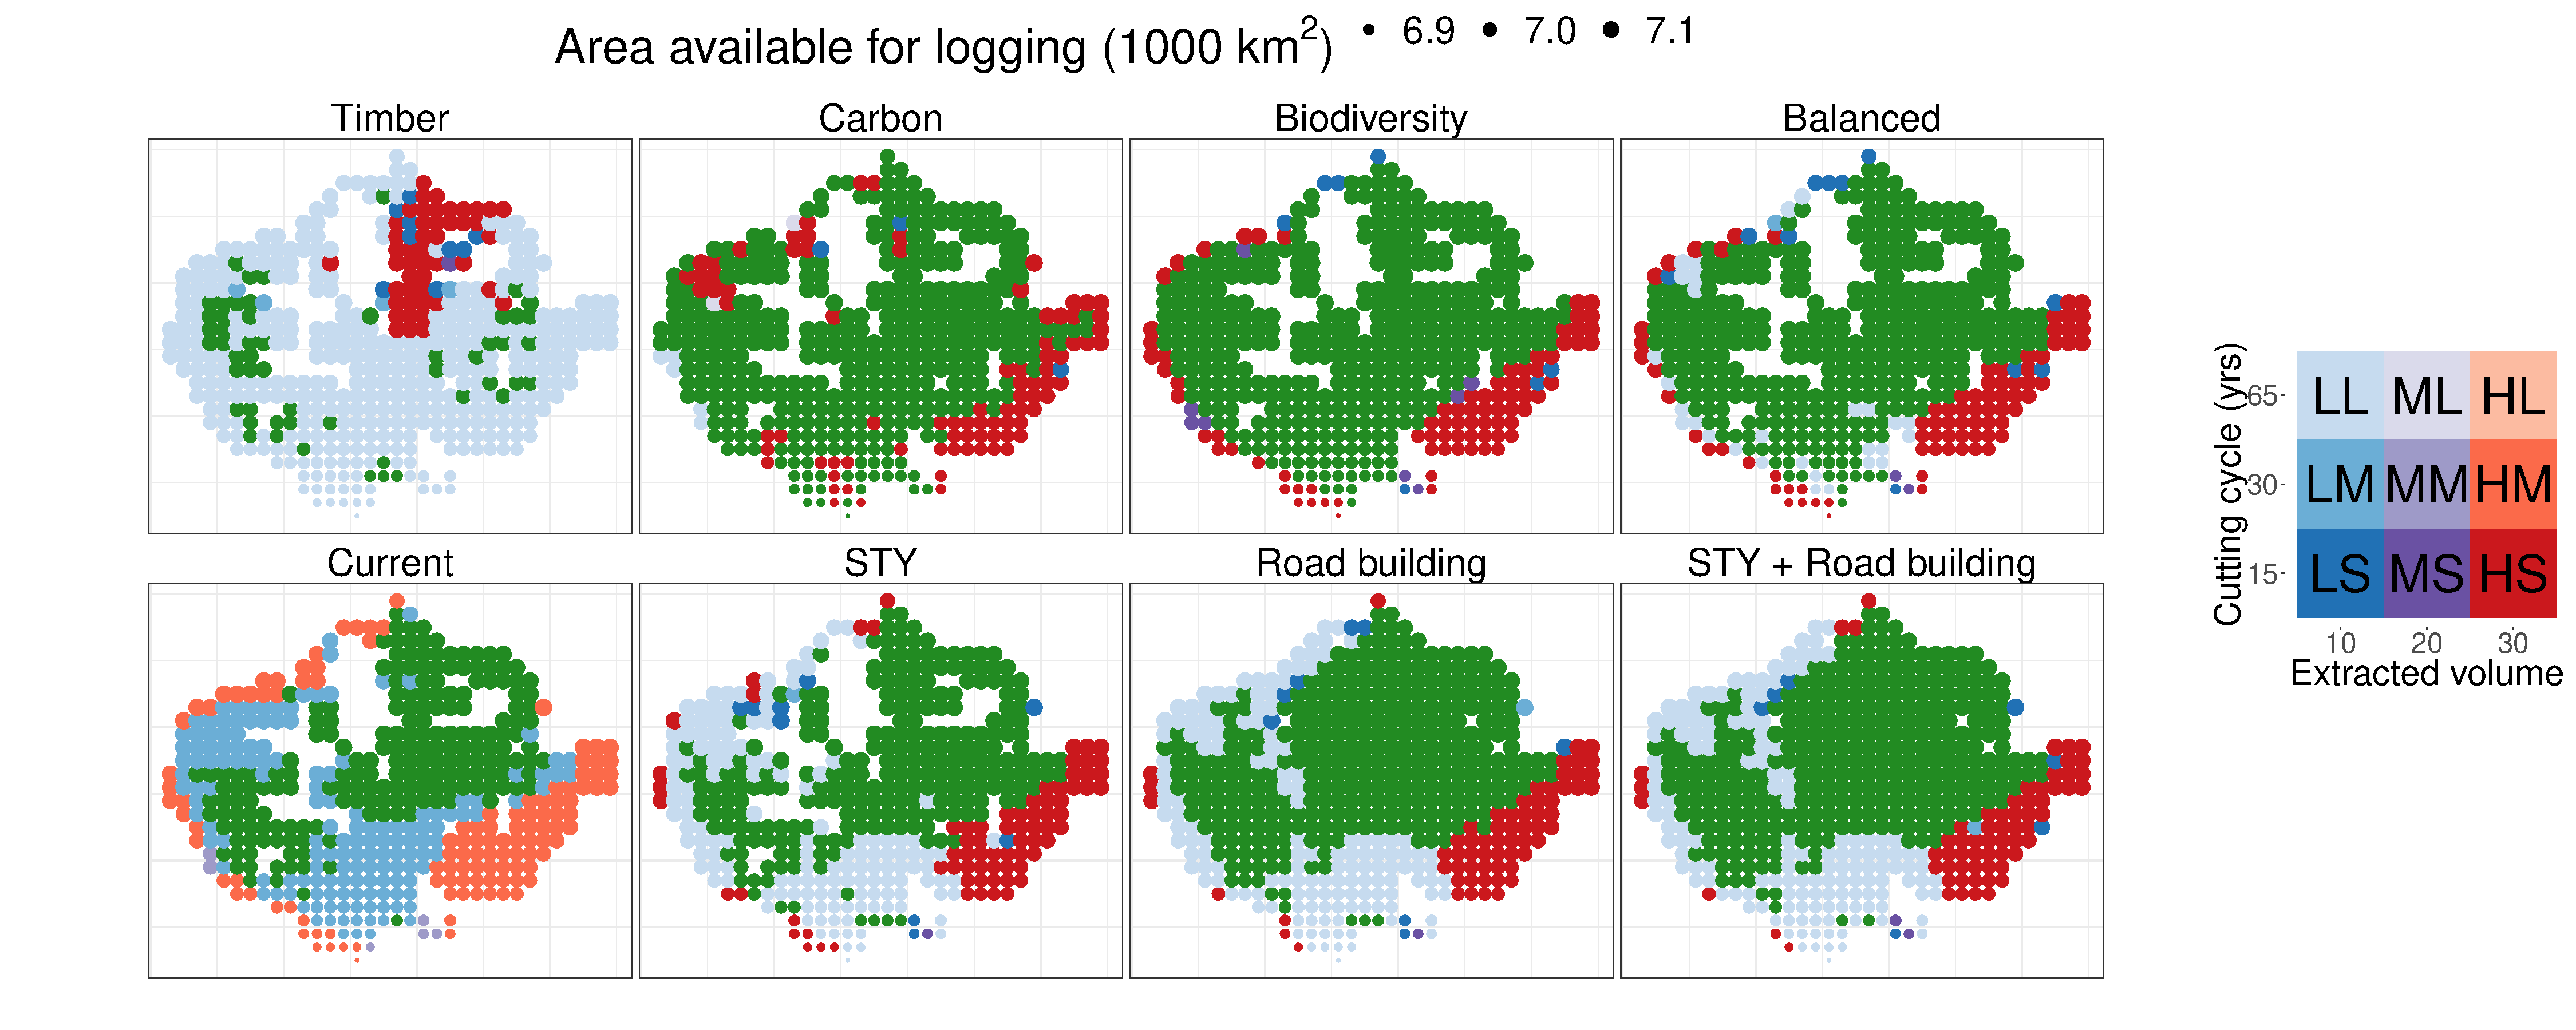
\includegraphics[width=0.8\linewidth]{graphs/mapsScenarios.pdf}
    \caption{Results of spatial optimisation with the 8 strategies defined in Table~\ref{tab:strategies}. Production target is set to 35~Mm$^3$yr$^{-1}$. Green areas are not logged. The size of each dot is proportional to the PPF area (total area available for logging). Logging type colour (blue - purple - red) represent the logging intensity (Light: 10, Medium: 20 and High: 30~m$^3$ha$^{-1}$). The logging type transparency represents the cutting cycle length (Short: 15, Medium: 30, Long: 65 years): light colours correspond to longer cycles.}
    \label{fig:mapsStrateg}
\end{figure*}

\subsection{Effect of strategy choice on ES provision}

The \textit{Timber} strategy results in the best final timber stocks (+1.4\% of initial timber stocks, Figure~\ref{fig:scenESProv}a) but the highest carbon emissions (-3.6\% of initial carbon stocks, Figure~\ref{fig:scenESProv}b) and highest biodiversity loss (-5.8\% of initial value, Figure~\ref{fig:scenESProv}c). The \textit{Carbon} and \textit{Biodiversity} strategies both result in high timber losses (-2.2\%), but low carbon emissions (-1.5\% and -1.6\% respectively) and low diversity losses (-2.4\% and -2.2\% respectively). 

The \textit{Balanced} and \textit{STY} strategies result in almost no variation in timber stocks while the \textit{Road building} and \textit{STY + Road building} strategies result in a timber increase of 0.8\% (Figure~\ref{fig:scenESProv}a). Those 4 strategies have similar carbon and biodiversity losses: -2.3\% carbon (Figure~\ref{fig:scenESProv}b) and -3.6\% biodiversity (Figure~\ref{fig:scenESProv}c) in the \textit{Balanced} and \textit{STY} strategies, and -2.2\% carbon and -3.7\% biodiversity in the \textit{Road building} and \textit{STY + Road building} strategies. 

The \textit{Current} strategy performs poorly at providing all ESs: it shows the highest loss of timber (-2.3\%) and the second highest losses of carbon (-3.5\%) and biodiversity (-4.9\%), not far behind the \textit{Timber} strategy. 

\subsection{Effect of change in timber production target}

The effect of changing the timber demand (timber production target from 10 to 80 Mm$^3$) was tested on the 8 management strategies.

For all strategies except one (the \textit{Timber} strategy), the total area harvested increases with the total production target (Figure~\ref{fig:incDemand}a). 
In the \textit{Timber} strategy however, the total area logged is at its maximum value (around 80 Mha) even for low production targets: the increase in timber production results in an increase in the mean logging intensity and in a decrease in the mean cutting cycle length (Figure~\ref{fig:incDemand}b-c). 
Provision of ESs (carbon, biodiversity, and timber) decreases when production increases (Figure~\ref{fig:incDemand}d-f).

The \textit{Carbon} and \textit{Biodiversity} strategies have similar behaviours: they rely almost exclusively on high-intensity (30~m$^3$ha$^{-1}$) short-cycle (15 yr) logging independently of the timber production target (Figure~\ref{fig:incDemand}b-c), and the  additional timber production target is met through an linear increase in logged areas (Figure~\ref{fig:incDemand}a). 

When ES prioritisation is balanced (\textit{Balanced} and \textit{Road building} strategies), timber production is mostly done under low-intensity long-cycle logging when the production target is low. The total area logged increases slowly with the timber production target (Figure~\ref{fig:incDemand}a): the additional timber is mostly produced by gradually substituting low-intensity long-cycle logging with high-intensity short-cycle logging (Figure~\ref{fig:incDemand}b-c; Figure~\ref{fig:mapsIncDemand}). 

Adding the STY constraint to the \textit{Balanced} and \textit{Road building} strategies (respectively the \textit{STY} and \textit{STY + Road building} strategies) does not change results when production target is low; when the timber stocks variation becomes negative however (at 35 Mm$^3$yr$^{-1}$ and 50 Mm$^3$yr$^{-1}$ respectively, Figure~\ref{fig:incDemand}d), the mean logging intensity plateaus at approximately 15~m$^3$ha$^{-1}$ and the mean cutting cycle stabilises at 50 years for both the \textit{STY} and \textit{STY + Road building} strategies. Intensifying logging or shortening cutting cycles would result in a net loss of timber stocks. The additional production target is then met through a sharp increase in the total area logged (Figure~\ref{fig:incDemand}a), until there is no more area available for logging. The STY constraint cannot be satisfied above 50 Mm$^3$yr$^{-1}$ with currently available PPF (i.e. in the \textit{STY} strategy) and 60 Mm$^3$yr$^{-1}$ with all potential PPF (i.e. in the \textit{STY + Road building} strategy). 

Finally, the \textit{Current} strategy (i.e. balanced ES prioritisation with cutting cycles of 30 years) results in low-intensity logging when the production target is under 20 Mm$^3$yr$^{-1}$ (Figure~\ref{fig:incDemand}b); increasing the timber production target results in a sharp increase in the total area logged until 30~Mm$^3$yr$^{-1}$ (Figure~\ref{fig:incDemand}a) and in a sharp increase in the logging intensity from 30~Mm$^3$yr$^{-1}$ to 80~Mm$^3$yr$^{-1}$ (Figure~\ref{fig:incDemand}b). When the timber production target reaches 80~Mm$^3$yr$^{-1}$, the total area logged reaches its maximum value (around 80~Mha; Figure~\ref{fig:incDemand}a) and all areas logged are under high-intensity logging (30~m$^3$ha$^{-1}$; Figure~\ref{fig:incDemand}b). In terms of ES provision, the \textit{Current} strategy performs poorly compared to other strategies, especially when the production target is high: it results in the highest timber, carbon and biodiversity losses when the timber production target reaches 35, 40, and 50~Mm$^3$yr$^{-1}$ respectively.  

\begin{figure*}
    \centering
    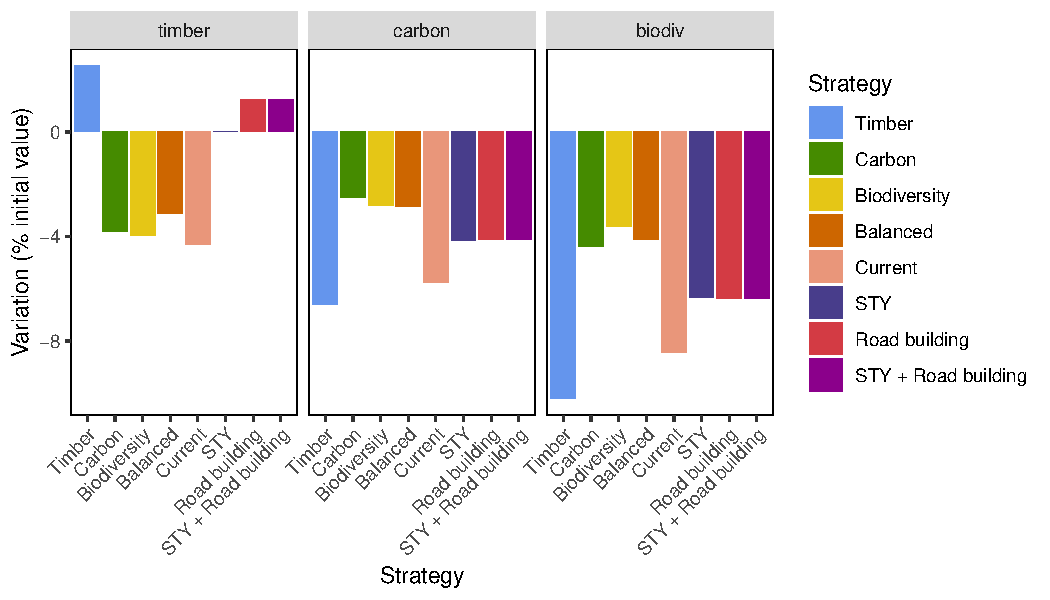
\includegraphics[width=\linewidth]{graphs/costsScenario}
    \caption{Impact of the 8 management strategies (described in Table~\ref{tab:strategies}) on ES provision (\% of the initial ES value). The timber production target is set to 35~Mm$^3$. (a) Variation of timber stocks; (b) variation of carbon stocks; (c) variation of biodiversity. A positive value indicates an increase in total ES provision; a negative value indicates a loss in total ES provision.}
    \label{fig:scenESProv}
\end{figure*}

\begin{figure*}
    \centering
    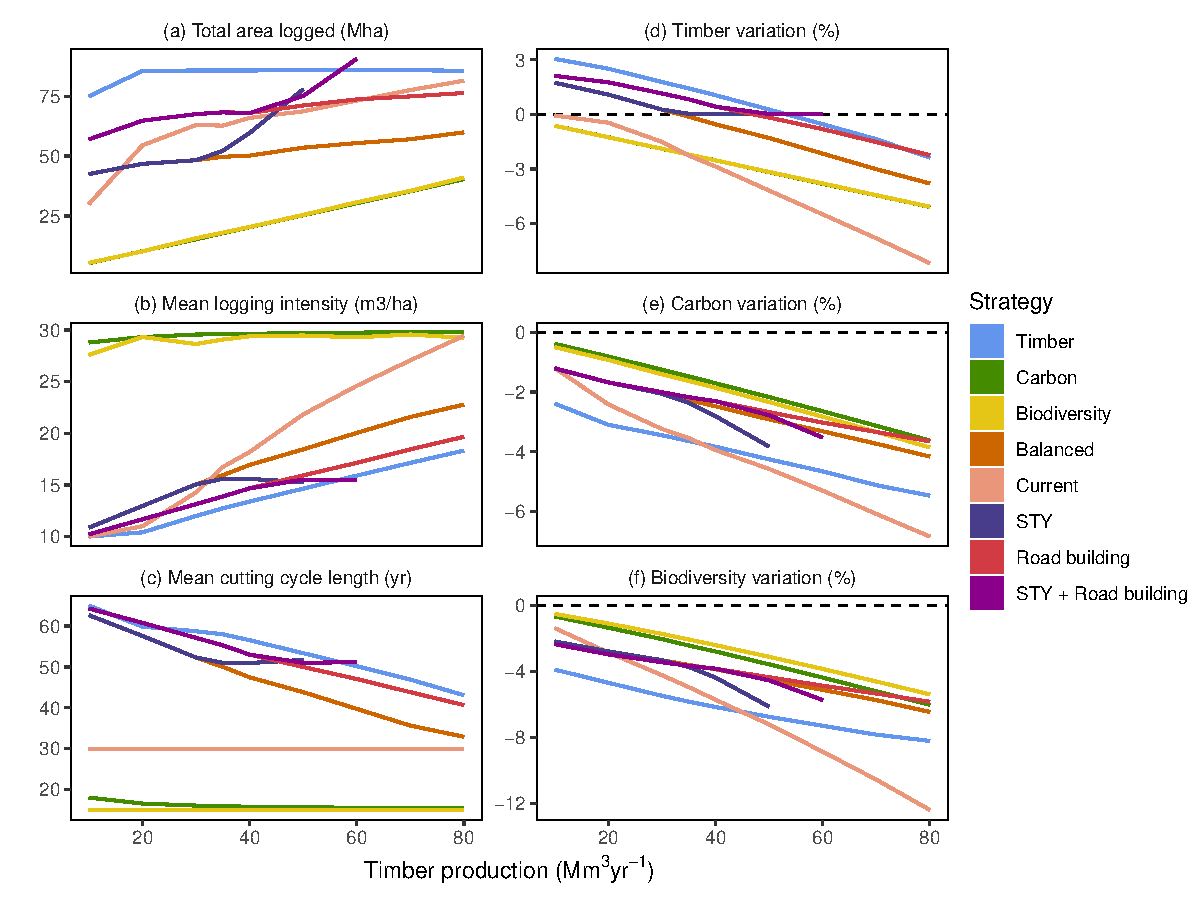
\includegraphics[width=\linewidth]{graphs/increasingDemand.pdf}
    \caption{Characterisation of different strategies for timber production, depending on the timber production target. (a) Total area logged (Mha). (b) Mean logging intensity in logged areas (m$^3$ha$^{-1}$). (c) Mean cutting cycle length (yr). (d) Variation of timber stocks (\% of the initial value). (e) Carbon emissions (\% of the initial value) (f) Variation of biodiversity value (\% of the initial value). The 8 strategies' characteristics are summarised in Table~\ref{tab:strategies}. \textit{STY} and \textit{STY + Road building} strategies could not sustainably provide more than 50 and 60 Mm$^3$ of annual timber production respectively. In plots (d-f), values are calculated over all areas outside of protected areas. Additional maps with distribution of logging types (intensity, cutting cycle) are provided in the supplementary material (Figure~\ref{fig:mapsIncDemand}).}
    \label{fig:incDemand}
\end{figure*}

\section{Discussion}

\subsection{Importance of regional studies for forest management}

The optimisation approach applied in this study can have many implications for forest management. Ecosystem services in selectively logged forests have often been studied but usually, they were analysed separately \cite{Putz2012}: there has been little investigation on the trade-offs that exist between ESs. Among the few studies that exist on the subject, a trade-off between carbon retention and timber recovery has been shown at the local scale, where those trade-offs depend on the logging intensity and silvicultural treatments applied \cite{Roopsind2018}. Trade-offs have also been reported between timber production and species richness \cite{Burivalova2014}.  
Local studies can inform forest owners, but the latter will base their decisions on a limited set of locally-relevant objectives. Their goal is usually to maximise financial benefits, may it be through timber or non-timber forest products harvesting, eco-tourism or payments for ecosystem services. 

Climate change mitigation and nature conservation goals are however more relevant at regional to global scales \cite{Hein2006b}: e.g. delimitation of protected areas and forest concessions \cite{Verissimo2002}, definition of logging rules (maximum logging intensities, unique cutting cycle length, minimum cutting size, protected tree species) \cite{Blaser2011}, road planning \cite{Laurance2014}. Informing these policies with large-scale multicriteria analyses will thus be key to develop evidence-based policies. Today few studies have assessed regional-scale ESs trade-offs in Amazonia (e.g. a recent study analyses tradeoffs between forest conservation and agriculture at the basin scale \cite{OConnell2018}); to our knowledge, none has focused on Amazonian forests managed for timber production. Our study is thus an important step in the planning of future logging management in Amazonia, that needs to be informed on where and how logging should be done depending on future demand for timber and other ESs. 

One important point to bear in mind is that results presented here only account for the first cutting cycle: this is particularly important in the sustained-timber-yields strategy because even though yields are sustained during the first cutting cycle they could decrease afterwards. Today there is almost no data on multi-cycle logging in Amazonia: most monitored plots have been logged only once \cite{Sist2015}, although actual logging in Amazonia may comprise multiple illegal reentries \cite{Tritsch2016a}. Gathering more information on the effect of several cutting cycles on forest dynamics will be of utmost importance to understand what future production forests will look like. 

We also did not include in the analysis potential benefits of the set of improved logging techniques gathered under the name of Reduced Impact Logging (RIL). A compelling body of evidence shows that RIL practices could provide large improvements in terms of timber recovery, carbon emissions and biodiversity protection \cite{Putz2008c,West2014,Tobler2018,Griscom2019}, and many authors thus argue that they should be an essential point in forest management strategies \cite{Runting2018}. Despite this long-standing research, RIL techniques are seldom implemented in Amazonian production forests \cite{Blaser2011}. We thus decided to base our study on currently dominant logging practices, keeping in mind that ES provision would be improved if RIL was more widely implemented. 

Finally, even though our findings provide an interesting insight on potential trade-offs that future forest managers and decision-makers will face, a large part (20-60\%) of logging is done illegally in the Amazon \cite{Finer2014,Brancalion2018}. Changing logging rules to maintain the environmental value of production forests can be jeopardised by the lack of control over their application. Improving Amazonian forests' governance will be key to maintain ecosystem services through informed management. 

\subsection{How to improve ES provision in production forests?}

The main strategy for maintaining high ES provision in production forests has been so far to implement logging rules that limit the cutting cycle length (20-65 years) and the logging intensity (20-30 m$^3$ha$^{-1}$) \cite{Blaser2011}. 
Those logging rules were thought as a compromise between producing enough timber to make financial benefits, and letting the forest recover long enough to make logging sustainable \cite{Seydack2012}.
Several studies showed however that current logging rules are not enough to recover pre-logging forest characteristics \cite{Zimmerman2012}.
Moreover, our results show that implementing intermediate logging rules leads to sub-optimal management of production forests: 30-yr cutting cycles and medium intensities (20~m$^3$ha$^{-1}$) are virtually never selected in the optimisation process (Figure~\ref{fig:mapsStrateg}), and a restriction to 30-yr cutting cycles increases the loss of all ESs (cf. the \textit{Current} strategy in Figure~\ref{fig:incDemand}d-f).  

The spatial configuration of optimal logging (Figure~\ref{fig:mapsStrateg}) highlights major regional differences in Amazonian forests. Forests of the Guiana Shield (northeastern Amazonia) are less prone to natural disturbances \cite{Espirito-Santo2014} and have thus adapted to those environmental conditions with low turnover rates and slow-growing species \cite{Johnson2016,Quesada2012}. 
Because they recover timber slowly, they are not logged when the demand for timber is low (see Supplementary material, Figure~\ref{fig:mapsIncDemand}). 
When the demand for timber is high, however, Guiana shield forests are allocated to high intensity logging when timber recovery is optimised (Figure~\ref{fig:mapsStrateg}c): in this case the high logging intensity is predicted to decrease the forest maturity, thus making the forest more productive \cite{Piponiot2018,Roedig2018,Perez-Espana1999}.

Nevertheless, Guiana shield forests provide other ESs: they harbour large amounts of carbon \cite{Avitabile2016} and vertebrates diversity \cite{Jenkins2013}, and are thus not selected for logging when biodiversity and carbon are optimised (Figure~\ref{fig:mapsStrateg}a-b). 
Additionally, other studies have found that forests of the Guiana Shield also play a crucial role in the Amazonian hydrological cycle \cite{Staal2018,Bovolo2018}, enhancing the importance of their conservation in future management strategies. 
As for the Guiana Shield, northern and central Amazonian forests harbour high levels of vertebrates diversity \cite{Jenkins2013} and carbon \cite{Avitabile2016} and are thus rarely selected for logging in this study when biodiversity conservation and carbon storage are prioritised (Figure~\ref{fig:mapsStrateg}a-b). If conservation is the main objective of Amazonian forest management, the consolidation of the protected area network in central and northeastern Amazonian forests will provide high benefits for conservation and climate change mitigation, especially if this promotes a higher connectivity between existing protected areas \cite{Hansen2007}. 

Southeastern forests, in turn, have lower levels of diversity and carbon. They are thus often allocated to high-intensity short-cycle logging when carbon and biodiversity are optimised (Figure~\ref{fig:mapsStrateg}a-b). 
However, because of previous forest degradation in the region through fire events, logging and forest fragmentation \cite{Foley2007,Davidson2012}, that affect particularly large trees \cite{Laurance2000,Gerwing2002}, the timber productivity may have been overestimated, even with closed canopies \cite{Asner2004}. Restoring degraded forests through silvicultural interventions may be an opportunity to increase timber yields \cite{Lamb2005}, but such interventions are costly and will require to adopt policies and financial incentives, e.g. through payments for ecosystem services \cite{Salzman2018}.

\subsection{Land-use strategies, trade-offs and implications for policy-making}

Our results reveal that the main trade-off is between a long-term provision of timber and forest conservation for carbon (climate change mitigation) and biodiversity (Figure~\ref{fig:changeCosts}). These results fit into the "land sharing vs land sparing" debate: with a given timber demand, should logging focus on intensely-logged areas and conserve the rest as intact forest, or should it use the entire landscape under low-intensity logging? Edwards and colleagues \cite{Edwards2014} showed that land-sparing logging retained higher levels of biodiversity in a Bornean forest concession. Because land-sparing logging creates heterogeneous landscapes and maintains higher levels of $\beta$-diversity, it has a higher potential for maintaining biodiversity at the landscape scale \cite{DeCastroSolar2015}. 
In the Indonesian province of East Kalimantan, a recent study found that optimal forest conservation value would be attained with land-sparing timber production (acacia plantations and protected areas) with some level of land-sharing (reduced-impact low-intensity) logging, where logging concessions act as buffers between conservation and production areas \cite{Runting2018}. 
Our findings also show that land-sparing logging not only minimises biodiversity loss (Figure~\ref{fig:mapsStrateg}b, Figure~\ref{fig:incDemand}f), but it can also reduce carbon emissions (Figure~\ref{fig:mapsStrateg}a, Figure~\ref{fig:incDemand}e). 
However the land-sparing strategy performs rather poorly in terms of timber recovery (Figure~\ref{fig:changeCosts}d), compared to a land-sharing strategy (e.g. the \textit{Timber} strategy, Figure~\ref{fig:incDemand}d). 

There seems to be little place for a win-win strategy between timber production and forest conservation, and the current strategy of intermediate logging rules leads to increased ES loss (Figure~\ref{fig:incDemand}d-f). The fate of Amazonian production forests should thus depend on political choices and on future societal demand for ESs. If maintaining long-term timber supply from natural forests is thought to be the goal \cite{Zarin2007}, then low-intensity logging should be widely applied in the Amazon, especially in the western part of the basin (Figure~\ref{fig:mapsStrateg}c).
However, if the societal demand to preserve carbon and biodiversity continues to increase (e.g. carbon-based policies like REDD+ \cite{Stickler2009}, or the 1992 Rio convention on biodiversity \cite{Barton1992}), then policies should focus on conserving intact inland forests while allowing high-intensity logging in the skirts of the Amazon basin. This type of policy will result in a fast depletion of timber stocks in those over-harvested forests. Alternative ways of producing timber, such as active forest restoration with intensive silviculture and mixed-species timber plantations \cite{Lamb2005}, should then be implemented in the meantime, in order to have new productive forests once the over-harvested forests are depleted. 

Interestingly, the \textit{Road building} and the \textit{Balanced} strategies, which only differ in terms of area accessible for logging (Table~\ref{tab:strategies}), give similar results in for biodiversity and carbon conservation (Figure~\ref{fig:incDemand}e-f), and road building provides only little improvement in terms of timber stocks recovery.
Building new roads (i.e., in the \textit{Road building} strategy) gives more options for the choice of logged grid cells, and thus increases ES provision (Figure~\ref{fig:incDemand}d-f), but the difference is small. 
Yet, logging roads open the forest to other uses, like hunting, wood-fuel harvesting and deforestation, which can increase carbon and biodiversity costs \cite{Laurance2009a}. Depending on the level of governance, forests can undergo long-lasting additional degradation that was not accounted for in this study but could increase the environmental cost of road-building strategies. Overall, building new roads to increase the area of production forests in Amazonia may not be a good strategy for future ESs provision. 

\section{Conclusion}

This study shows that large-scale trade-offs exist between maintaining timber stocks and maximising biodiversity and climate change mitigation in Amazonian production forests. Land-sharing strategies that promote low-intensity logging in entire regions of the Amazon basin will result in sub-optimal biodiversity and high carbon emissions at the regional level, but land-sparing strategies that maximise global forest conservation will result in timber depletion of highly logged areas, and will thus require finding alternative timber sources in the future. Applying intermediate logging rules, e.g. 30-yr minimum cutting cycles, only results in sub-optimal ES provision. Our results stress the need for a concerted reevaluation of current logging rules in Amazonia, and the importance of management choices for future production forests depending on societal demand for ecosystem services. 

\clearpage

\bibliographystyle{nature}
\bibliography{biblio}


\onecolumn
\beginsupplement
\appendix
\begin{center}
    { \huge \textbf{Supplementary material}}
\end{center} 

\section{Quantifying the effect of logging on ESs}
\label{sec:ESestimation}

\subsection{Timber production and recovery}

From a previously developed volume recovery model calibrated at the Amazonian scale \cite{Piponiotc}, we extracted: (i) the total volume $vtot_p$ (m$^3$ha$^{-1}$) in grid cell $p$, (ii) the proportion of potentially commercial timber $\omega 0_p$ and (iii) the potential timber recovery $vrec_{p,z}$ at the end of a cutting cycle $trot_z$ and after a logging intensity $vext_z$ ($z$ being the logging type). All parameters were set to their maximum likelihood value.

The mean annual timber production over the first cutting cycle in grid cell $p$ in logging type $z$ is equal to: 
\begin{equation}
\label{eq:prod}
    Prod_{p,z}  =  \frac{min\big(vext_z, (vtot_p\cdot \omega 0_p) \big) \cdot area_p}{trot_z}
\end{equation}

where $vext_z$ is the extracted volume in logging type $z$, $vtot_p\cdot \omega 0_p$ is the potential timber volume (the actual extracted volume cannot exceed the potential timber volume), $area_p$ is the area available for logging and $trot_z$ is the cutting cycle length.

The mean annual timber recovery over the first cutting cycle in grid cell $p$ in logging type $z$ is equal to: 

\begin{equation}
\label{eq:rec}
    Rec_{p,z} = \frac{vrec_{p,z}\cdot area_p}{trot_{p,z}}
\end{equation}

\subsection{Carbon emissions}

The effect of logging on carbon emissions is here quantified as the mean difference to the initial carbon stock over the cutting cycle. It was assessed as the difference of two terms: (i) the initial carbon loss caused by logging, (ii) minus the carbon storage from forest regrowth, averaged over the cutting cycle. 

The initial carbon loss caused by logging is threefold: (i) from extracted logs; (ii) from road building (deforestation), (iii) from incidental damage during logging operations \cite{Piponiot2016}. 

The carbon emissions from extracted logs in grid cell $p$ under logging type $z$ was assessed as: 

\begin{equation}
\label{eq:cext}
    Cext_{p,z} = Prod_{p,z} \cdot WDext_p \cdot  area_p
\end{equation}

with $Prod_{p,z}$ the actual logging intensity (in m$^3$ha$^{-1}$), $area_p$ is the area available for logging (ha) in grid cell $p$ and $WDext_p$ is the mean wood density of commercial trees in grid cell $p$ (see supplementary section~\ref{supmat:wdext} for wood density estimation). 

The carbon emissions from road building were estimated as follow: 

\begin{equation}
\label{eq:croad}
    Cdefor_{p,z} = Pdefor \cdot acs_p \cdot area_p
\end{equation}

where $Pdefor = 4.7 $\% is the estimated proportion of a logged area that is deforested for infrastructure (roads, logging decks and main skid trails) according to Piponiot et al. \cite{Piponiot2016} and $acs_p$ is the mean aboveground carbon density (MgC.ha$^{-1}$) in grid cell $p$, extracted from a global carbon map \cite{Avitabile2016}. 

Carbon losses from damaged trees were assessed as follows: 

\begin{equation}
\label{eq:cdam}
    Cdam_{p,z} = \frac{acs_p  - Prod_{p,z} \cdot WDext_p } {1 + \left(\frac{acs_p}{Prod_{p,z} \cdot WDext_p}  -1 \right)^\theta} \cdot area_p
\end{equation}

with $\theta$ a parameter of the model: the model justification and calibration are presented in supplementary section~\ref{supmat:cdam}. 

Post-logging carbon recovery $Crec_{p,z}$ was assessed with the methodology developed by Piponiot et al. \cite{Piponiot2016a}.  
All parameters were set to their maximum likelihood value. 

For each grid cell $p$ and each logging type $z$, the mean annual carbon emissions from grid cell $p$ under logging type $z$ are thus calculated as: 

\begin{equation}
\label{eq:cemi}
    Cemi_{p,z} = Cext_{p,z} + Cdefor_{p,z} + Cdam_{p,z} -  \sum_{t=1}^{trot_z} \frac{Crec_{t,p,z}}{trot_z} 
\end{equation}

\subsection{Biodiversity}

We chose to model the effect of logging on amphibians and mammals richness because they are key animals in forest ecosystems: amphibians are good indicators of global ecosystem health \cite{Welsh1998,Collins2003} and mammals ensure many ecosystem functions, among which pollination \cite{Fleming2009} and seed dispersal \cite{Wright2000,Muscarella2007}. We used global maps of mammals and amphibians richness derived from IUCN species range maps \cite{Jenkins2013,MapBiodiv}, which can fairly represent patterns of conservation priority \cite{Marechaux2017}.

The impact of logging on mammals and amphibians was assessed with the equation: 

\begin{equation}
\label{eq:rloss}
Rloss_{p,z} = \left(Rm_{p} \cdot \beta m + Ra_{p} \cdot \beta a  \right)  \cdot vext_z \cdot area_p 
\end{equation}

where $Rloss_{p,z}$ is the loss of vertebrate richness (mammals and amphibians) in grid cell $p$ and logging type $z$, $Rm_{p}$ and $Ra_p$ are the pre-logging richness of mammals and amphibians respectively \cite{Jenkins2013}, $\beta m = 1.44$ and $\beta a = 1.53$  are the estimated slopes of post-logging species loss in the Neotropics for mammals and amphibians respectively, according to Burivalova et al.  \cite{Burivalova2014}. $vext_z$ is the logging intensity in logging type $z$.
We hypothesize that amphibians and mammals richness do not recover after logging (no effect of cutting cycle length). 

\subsection{Wood density estimation}
\label{supmat:wdext}

\begin{figure*}
    \centering
    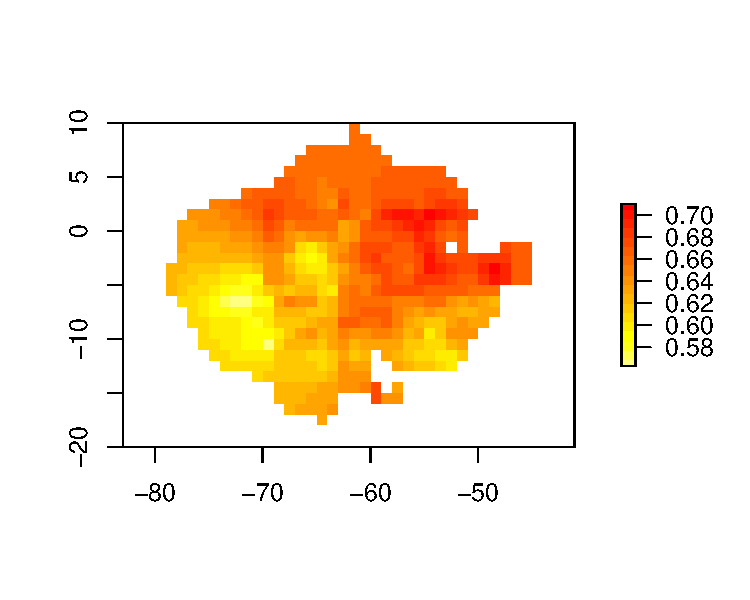
\includegraphics[width=0.7\linewidth]{graphs/map_WDext.pdf}
    \caption{Map of predicted wood density from interpolation of RadamBrasil data}
    \label{sfig:wdext}
\end{figure*}

We used 2646 1-ha forest inventory plots spanned over the Brazilian Amazon from the RadamBrasil project \cite{Radam2017}, in which all trees $\geq$33 cm diameter at breast height (DBH) were measured, identified to the species level and had their volume estimated. 

In every plot we estimated the mean wood density of all commercial stems (as defined in a previous study \cite{Piponiotc}) with the R package BIOMASS \cite{Rejou-Mechain2017}.
Values were then interpolated with the R package \textit{automap} \cite{gstat} on a 1$^{\circ}$ resolution grid (Supplementary figure~\ref{sfig:wdext}).


\subsection{Carbon damage model}
\label{supmat:cdam}

\begin{figure}
    \centering
    \begin{subfigure}[b]{0.3\textwidth}
        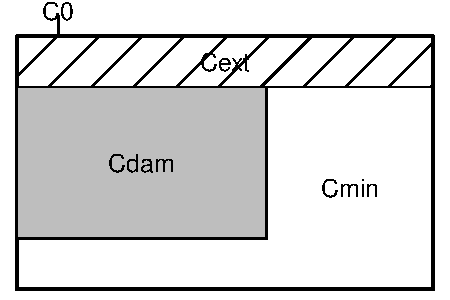
\includegraphics[width=\linewidth]{graphs/schemaDam.pdf}
        \caption{Diagram of carbon pools in the damage model.}\label{fig:schemaDam}
    \end{subfigure}
    ~ 
    \begin{subfigure}[b]{0.55\textwidth}
    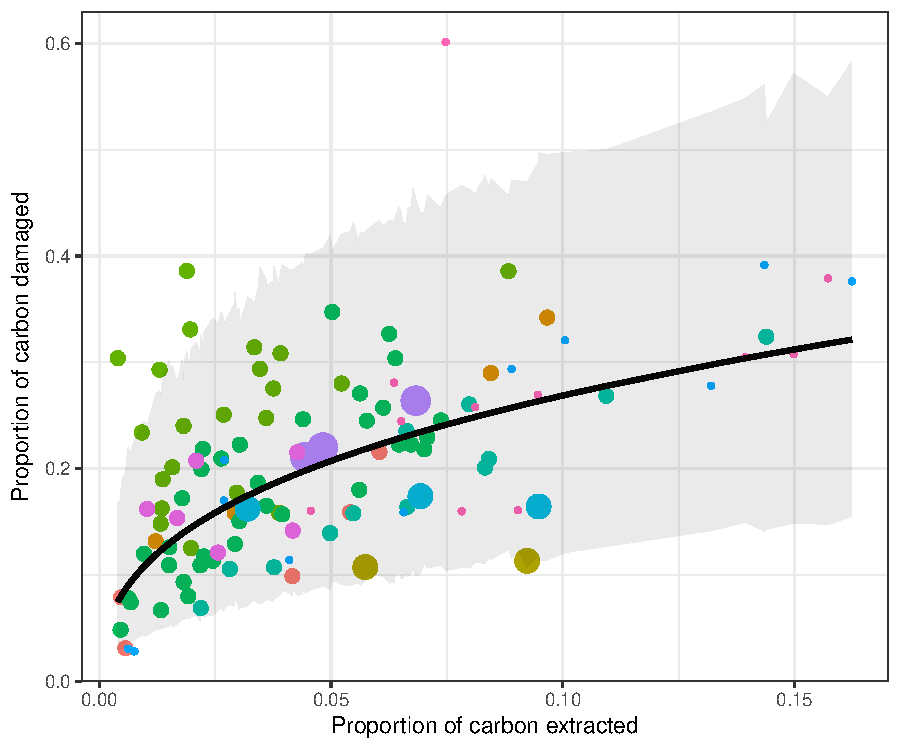
\includegraphics[width=\linewidth]{graphs/damModel.pdf}
    \caption{Carbon damage model. Coloured dots are data from one plot, with each colour representing one site and the size of the dot being proportional to the plot's size. The black line is the maximum likelihood prediction, and the shaded area is the 95\% confidence interval.}\label{fig:damModel}
    \end{subfigure}
\end{figure}

To estimate carbon emissions from logging damage we calibrated a model with data from 115 plots (129.25~ha total) in 11 experimentally logged sites spread in Amazonia \cite{Sist2015}. In all plots the identity of harvested trees was recorded, and at least one pre-logging and 2 post-logging forest inventories were carried out. In each forest inventory the diameter at breast height (DBH) of all stems $>$~20 cm DBH were measured, and trees were identified to the lowest taxonomic level (83\% species, 16\% genus, 2\% not identified). 
From forest inventories the above ground carbon and wood density of all trees $>$ 20 cm DBH  were estimated with the R package BIOMASS \cite{Rejou-Mechain2017}. 

The carbon extracted from plot $j$ was estimated as: 

\begin{equation}
    Cext_j = \sum_{i} \underbrace{a_j \cdot DBH_i^b}_{\text{volume of tree $i$}} \cdot WD_i
\end{equation}

with $DBH_i$ is the DBH of the logged tree $i$, $WD_i$ is its wood density and $a_j$, $b$ are the two parameters of a volumetric equation calibrated at the Amazonian scale \cite{Piponiotc}. 

The carbon of damage was estimated as: 

\begin{equation}
    Cdam_j = C0_j - Cext_j - Cmin_j
\end{equation}

where $C0_j$ is the pre-logging above ground carbon of all trees $>$ 20 cm DBH in plot $j$, and $Cmin_j$ is the minimum above ground carbon during the 4 years following logging operations (Figure~\ref{fig:schemaDam}). 

We define the following variables: 

\begin{itemize}
    \item $RatioExt_j=\frac{Cext_j}{C0_j}$ is the proportion of the initial above-ground carbon $C0_j$ that is extracted of the plot $j$; 
    \item $RatioDam_j = \frac{Cdam_j}{C0_j-Cext_j}$ is the proportion of damage in the carbon left in plot $j$ after logging operations. 
\end{itemize}

We calibrated the following model (see Figure~\ref{fig:damModel}): 

\begin{equation}
logit(RatioDam_j) \sim \mathcal{N}(\theta \cdot logit(RatioExt_j), \sigma_D^2)
\end{equation} 

with $\theta$ the slope of the relationship, and $\sigma_D$ the standard deviation. 


\clearpage

\section{Mapping potential production forest areas}

\label{sec:defPPF}

xxxx

\begin{figure}
    \centering
    \includegraphics{graphs/pp}
    \caption{Caption}
    \label{fig:my_label}
\end{figure}

\clearpage

\section{Analysing the effect of changing ES prioritisation}
\label{supsec:changeCost}

When optimising biodiversity (i.e. when biodiversity weight is 100\%), carbon emissions are 0\% higher than the optimal value (when optimising only carbon emissions, i.e. when carbon weight is 100\%: Figure~\ref{fig:changeCosts}) and timber loss is 34\% higher than the optimal value (Figure~\ref{fig:changeCosts}). When optimising carbon, biodiversity loss is 40\% higher than the optimal value (Figure~\ref{fig:changeCosts}) and timber loss is 37\% higher than the optimal value (Figure~\ref{fig:changeCosts}). When optimising timber, carbon emissions are 158\% higher than the optimal value (Figure~\ref{fig:changeCosts}) and biodiversity loss is 228\% higher than the optimal value (Figure~\ref{fig:changeCosts}).  When costs are balanced (carbon weight = biodiversity weight = timber weight), carbon emissions are 17\% higher than the optimal value (Figure~\ref{fig:changeCosts}), biodiversity loss is 11\% higher than the optimal value (Figure~\ref{fig:changeCosts}) and timber loss is 35\% higher than the optimal value (Figure~\ref{fig:changeCosts}). 

From this sensitivity analysis, one major trade-off axis emerges between carbon and biodiversity retention vs. timber recovery. 

\begin{figure*}
    \centering
    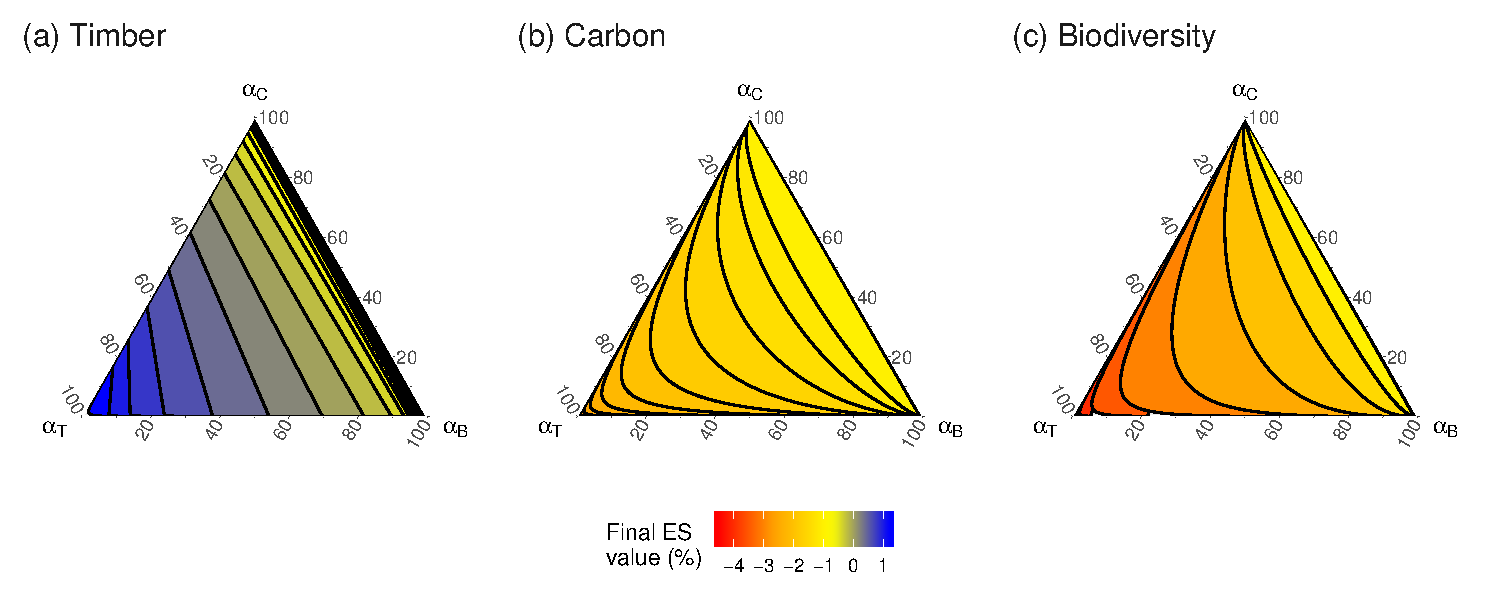
\includegraphics[width=\textwidth]{graphs/changingESweights.pdf}
    \caption{ES variation depending on the weight given to each ES in the optimisation process. $\alpha_T$, $\alpha_C$ and $\alpha_B$ are the weights given to timber, carbon and biodiversity, respectively (as a percentage of the total weight). Each ES variation is expressed as a proportion (\%) of the initial value for the corresponding ES. For example a carbon variation of -2\% means that total carbon emissions associated to logging correspond to 2\% of initial carbon stocks.} 
    \label{fig:changeCosts}
\end{figure*}


\clearpage

\begin{figure*}
    \centering
    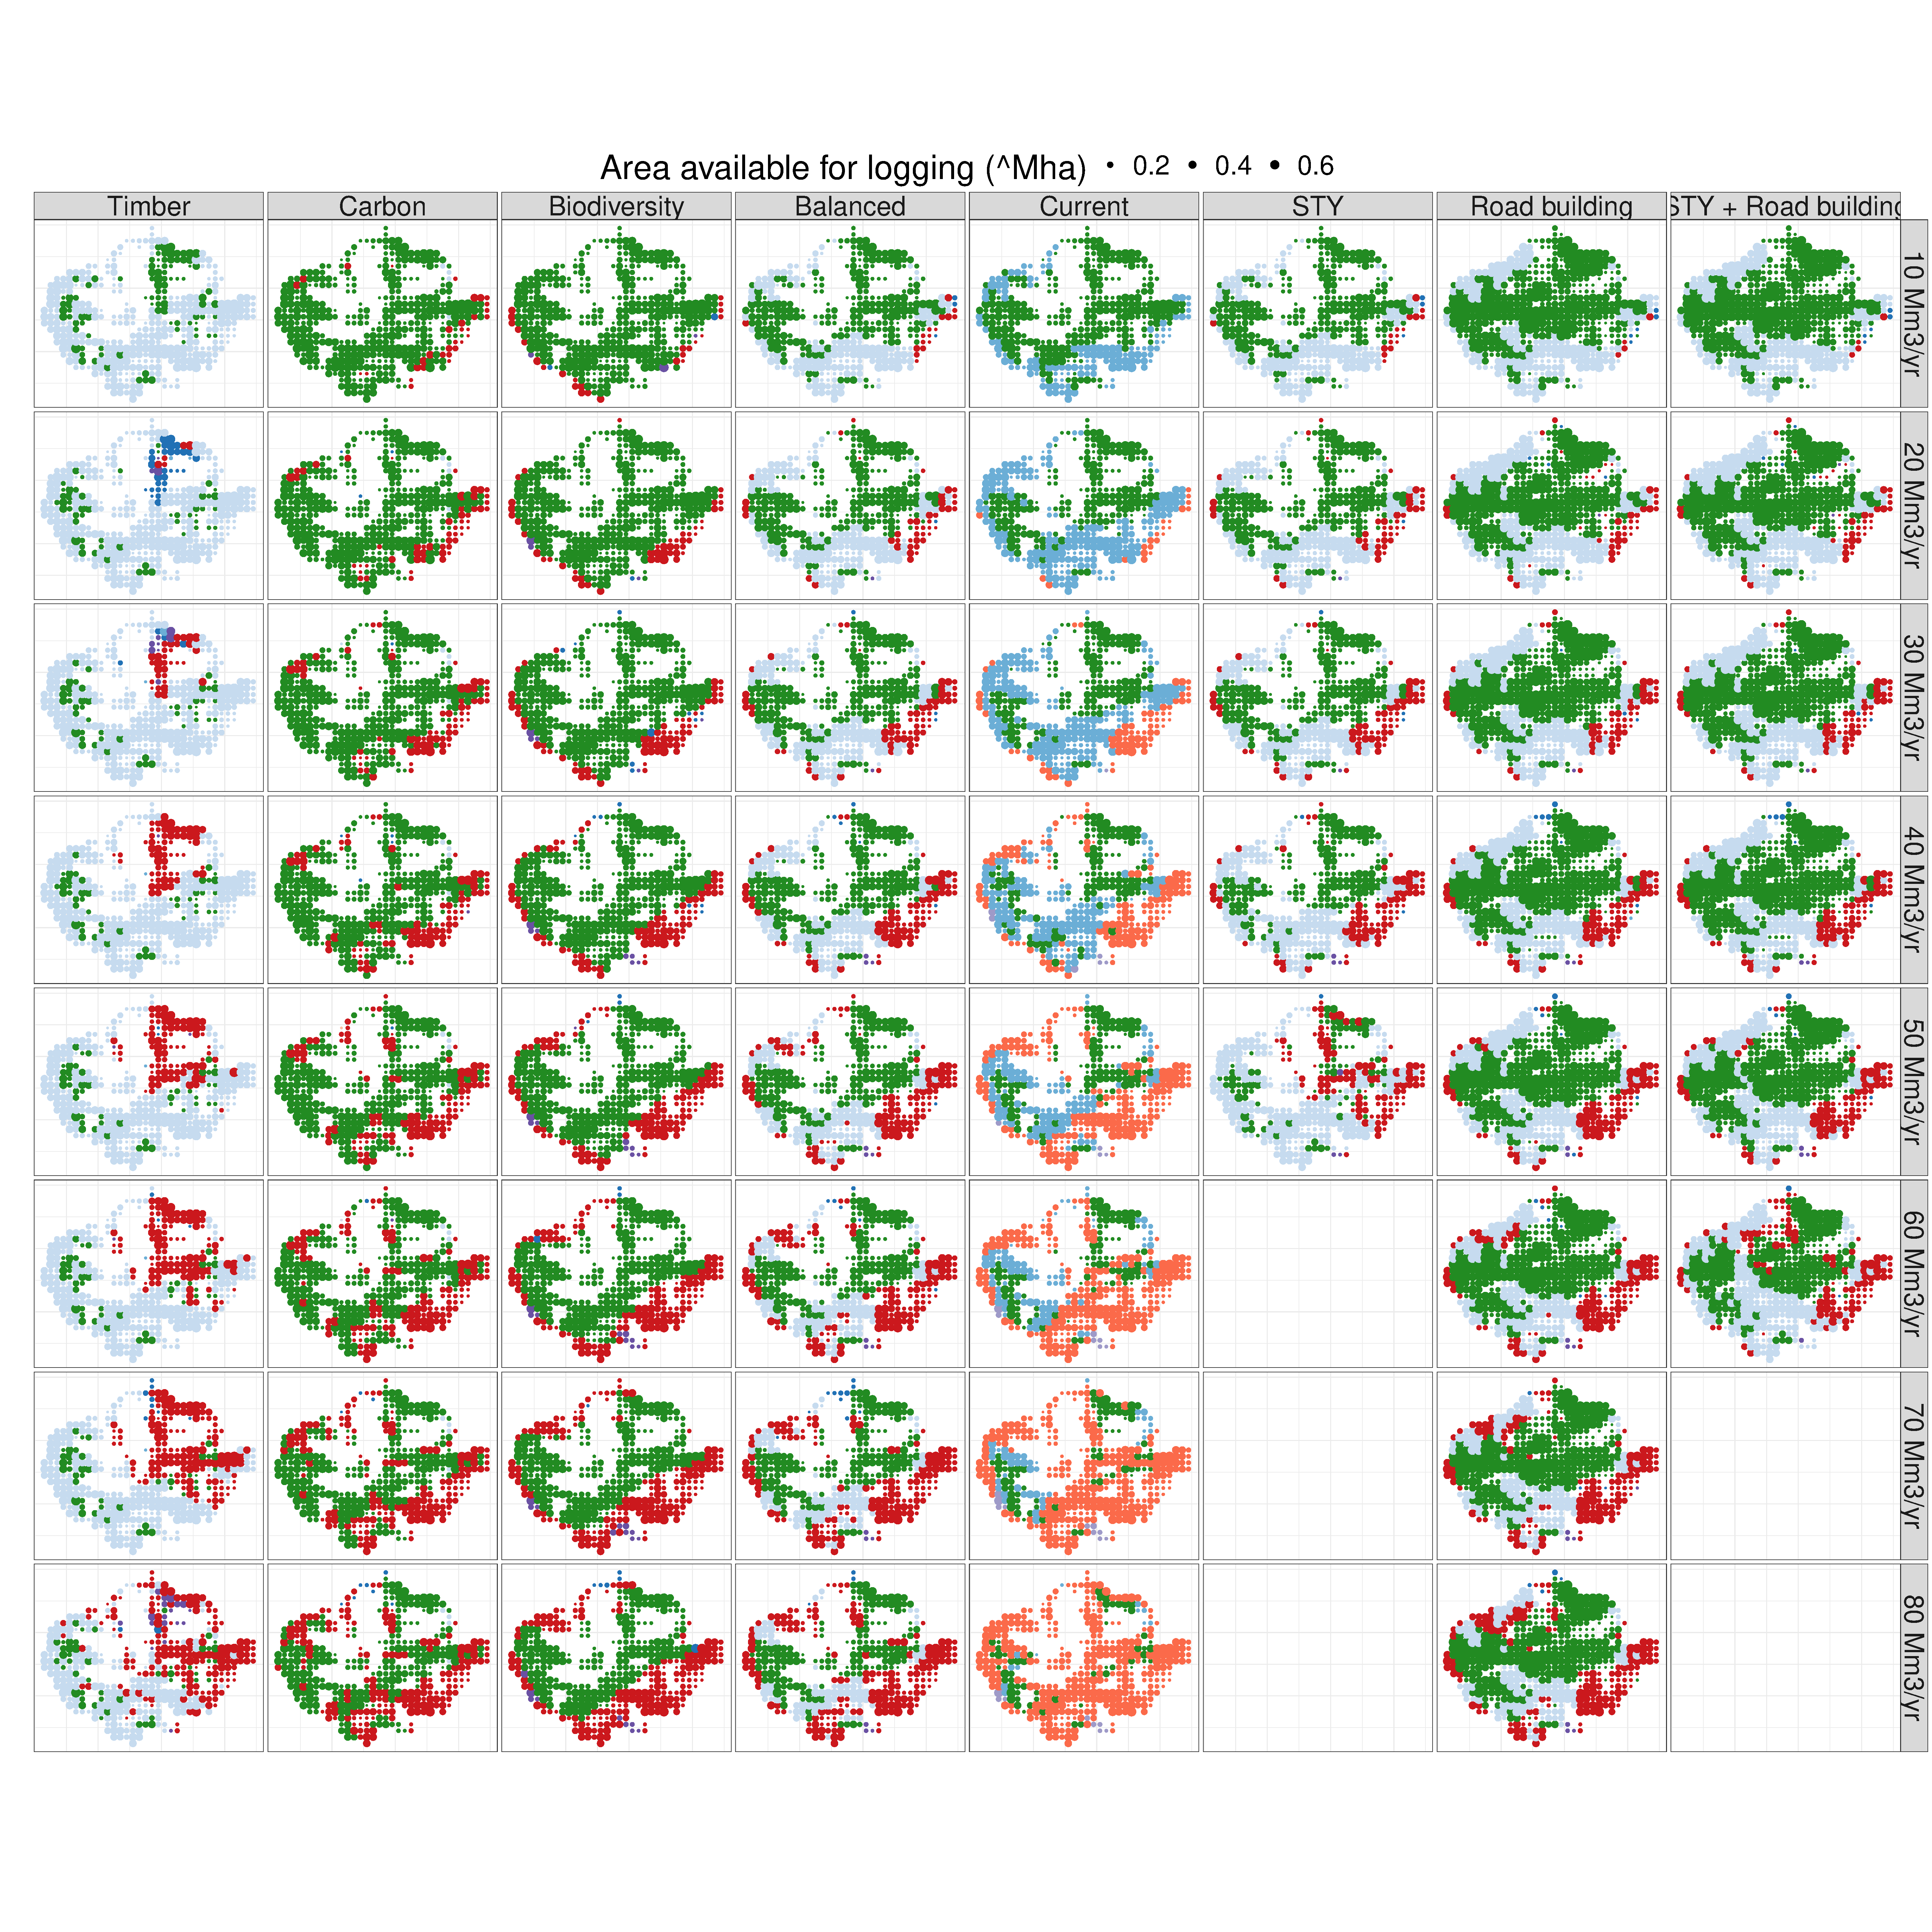
\includegraphics[width=\linewidth]{graphs/mapsChangeDemand.pdf}
    \caption{Results of spatial optimisation with varying demand for timber (from 10 to 80 Mm$^3$/yr), and under different scenarios.}
    \label{fig:mapsIncDemand}
\end{figure*}

\end{document}